\documentclass[10pt,unicode,notheorems]{beamer}

\usetheme[numbers, totalnumbers,minimal,nologo]{Statmod}
\usepackage[T2A]{fontenc}
\usepackage[utf8]{inputenc}
\usepackage[russian]{babel}
\usepackage{amsthm}
\usepackage{amsmath}
\usepackage{bm}
\usepackage{bbold}
\newtheorem{result}{Утверждение}
\newtheorem{theorem}{Теорема}
\newtheorem{lemm}{Лемма}
\newtheorem{remark}{Предложение}
\newtheorem{theorem+}{Теорема (Freund, Schapire, 1996)}
\DeclareMathOperator{\E}{E} 
\DeclareMathOperator{\T}{T} 
\DeclareMathOperator{\D}{D} 

\usepackage[scr]{rsfso}
\newcommand{\Laplace}{\mathscr{L}}

\begin{document}
\title{Композиция методов. Бустинг.}
\author{Романова Елизавета, Горбачук Анна, Сидоренко Денис}
%\institute[СПбГУ] {Санкт-Петербургский государственный университет \\
%    Прикладная математика и информатика \\
%    Кафедра статистического моделирования\\ } 

\date{
    Санкт-Петербург\\
    2019г.
}

\begin{frame}
    \titlepage
\end{frame}

\begin{frame}{Случайный лес.}
\begin{itemize}
    \item композиция большого количества глубоких деревьев;
    \item базовые алгоритмы (базовые решающие деревья) независимы.
\end{itemize}    
Проблемы:
\begin{itemize}
    \item обучение глубоких деревьев~--- трудоемкая процедура (построение деревьев ненаправленное, нужно много деревьев для сложных задач);
    \item если ограничить глубину, деревья улавливают не все группы.
\end{itemize}    
Пример: синий класс состоит из двух групп: одна в центре, одна с краю. Из-за того, что деревья очень небольшой глубины (в данном случае — 2), они могут уловить только одну из этих групп — ту, которая в центре, а на второй они полностью ошибаются.
\begin{figure}
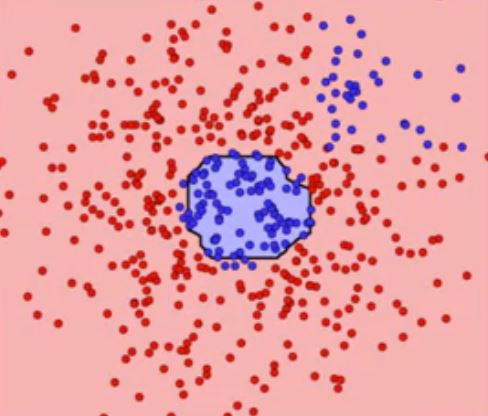
\includegraphics[width=0.3\linewidth]{trees.JPG}
\end{figure}
\end{frame}


\begin{frame}{Бустинг. Постановка задачи.}
\textbf{Бустинг:}
 \begin{itemize}
    \item последовательное обучение базовых алгоритмов;
    \item каждый следующий исправляет ошибки предыдущих;
    \item за счет этого достаточно простых базовых алгоритмов.
\end{itemize}   
\vspace{0.5cm}

\textbf{Постановка задачи:}

Пусть $X$ --- множество объектов, $Y$ --- множество ответов\\
$y: X \to Y$ --- неизвестная зависимость.

\vspace{0.2cm}
Дано: обучающая выборка --- $X^n = (x_i,y_i)_{i=1}^n $, \\
$y_i = y(x_i), i = 1,\ldots,n$ --- известные ответы.

\vspace{0.2cm}
Требуется построить алгоритм $a(x) = C(b(x))$, аппроксимирующий целевую зависимость $y$ на всём множестве $X$.
\end{frame} 

\begin{frame}{Изменение постановки задачи.}
   \textbf{Замечание:} вместо одного базового алгоритма $b$ рассматривается несколько алгоритмов $b_1(x), \ldots , b_T (x)$.
\vspace{0.2cm}

$\mathcal{B}(\Theta) = \{b(\cdot;\theta)|\theta \in \Theta \}$~---  параметризованное множество базовых алгоритмов.
\vspace{0.2cm}

Выбор базового алгоритма: выбор $\theta \in \Theta$ и $b(x)=b(x;\theta) \in \mathcal{B}(\Theta)$.
\vspace{0.2cm}

В качестве базовых алгоритмов обычно выступают:
\begin{itemize}
    \item решающие деревья (неглубокие 2-8) — используются чаще всего;
    \item пороговые правила (data stumps).
\end{itemize}
\vspace{0.2cm}

\textbf{Задача:} Подбор оптимальных (в смысле рассматриваемой функции потерь) базовых алгоритмов $\{b_t(x)\}_{t=1}^T$.
\end{frame}

\begin{frame}{Простой пример для задачи регресии.}
Хотим минимизировать среднеквадратичную ошибку
$$MSE(a,X) = \frac{1}{n} \sum \limits_{i=1}^n (a(x_i)-y_i)^2.$$
\begin{itemize}
    \item обучим простой алгоритм (неглубокое дерево): $b_1(x) = \arg \min \limits_{b \in \mathcal{B}} \frac{1}{n} \sum \limits_{i=1}^n (b(x_i)-y_i)^2$;
    \item хотим добавить еще один алгоритм $b_2$. Возникает вопрос: какие ответы $b_2$ должен давать на объектах обучающей выборки, чтобы ошибка нашей композиции была как можно меньше? \\
    \vspace{0.2cm}
    $b_1(x_i) + b_2(x_i) = y_i \Rightarrow $ \\
    \vspace{0.2cm}
    $b_2(x) = \arg \min \limits_{b \in \mathcal{B}} \frac{1}{n} \sum \limits_{i=1}^n (b(x_i)- (y_i-b_1(x_i)))^2$ \\
    $\ldots$ \\
    $b_T(x) = \arg \min \limits_{b \in \mathcal{B}} \frac{1}{n} \sum \limits_{i=1}^n (b(x_i)- (y_i- \sum \limits_{t=1}^T b_t(x_i)))^2$
\end{itemize}
\end{frame}   

\begin{frame}{Понятие композиции алгоритмов.}
Введем вспомогательное множество $R$, называемое пространством оценок. Будем рассматривать алгоритмы, имеющие вид суперпозиции $a(x) = C(b(x))$, где функция $b : X \to R$ называется \textbf {алгоритмическим оператором}, функция $C : R \to Y$ — \textbf{решающим правилом}.
\vspace{0.2cm}

\textbf{Композицией} $T$ алгоритмов $a_t(x) = C(b_t(x))$, $t = 1, \ldots, T$ называется суперпозиция алгоритмических операторов $b_t: X \to R$, корректирующей операции $F : R^T \to R$ и решающего правила $C : R \to Y$:
\begin{equation}
a(x) = C(F(b_1(x), \ldots , b_T (x)), \quad x \in X.
\end{equation}

Суперпозиции вида $F(b_1, \ldots , b_T)$ являются отображениями из $X$ в $R$, то есть алгоритмическими операторами.
\end{frame}


\begin{frame}{Пространство оценок. Примеры.}
Пространство оценок R вводится для того, чтобы расширить множество допустимых корректирующих операций.
\vspace{0.2cm}

\textbf{Пример 1.} В задачах классификации на два класса, $Y = \{-1, +1\}$, в качестве пространства оценок обычно используется множество действительных чисел $R = \mathbb{R}$.

В этом случае алгоритмические операторы называют также вещественнозначными
классификаторами: $C(b(x)) = sign b(x)$.
\vspace{0.2cm}

\textbf{Пример 2.} В задачах классификации на $M$ классов, $Y = \{1, \ldots , M\}$, в качестве пространства оценок обычно используется $R = \mathbb {R}^M$. Алгоритмический оператор $b(x)$ выдаёт вектор оценок принадлежности объекта $x$ каждому из классов, $b(x) = b^1(x), \ldots, b^M(x)$. 

Решающее правило $C$ относит объект к тому классу, для которого оценка максимальна:
$C(b(x)) \equiv C(b^1(x), \ldots, b^M(x)= \arg \max \limits_{y \in Y} b^y(x)$.
\vspace{0.2cm}

\textbf{Пример 3.} В задачах регрессии множество $Y$ уже достаточно богато, обычно $Y = \mathbb R$, поэтому использовать решающее правило нет особого смысла. В этом случае обычно полагают $R = \mathbb R$, $C(b) \equiv b$.
\end{frame}

\begin{frame}{Примеры корректирующих операций.}
\begin{itemize}
    \item \textbf{Пример 1.} Простое голосование (Simple Voting):
$$F(b_1(x), \ldots , b_T(x))= \frac{1}{T} \sum_{t=1}^{T} b_t(x), \quad x \in X.$$

 \item \textbf{Пример 2.}  Взвешенное голосование (Weighted Voting):
$$F(b_1(x), \ldots , b_T(x))= \sum_{t=1}^{T} \alpha_t b_t(x), \quad x \in X, \quad \alpha_t \in R.$$

 \item \textbf{Пример 3.}  Смесь алгоритмов (Mixture of Experts):
$$F(b_1(x), \ldots , b_T(x))= \sum_{t=1}^{T} g_t(x)b_t(x), \quad x \in X, \quad g_t: X \to  \mathbb R.$$  
\end{itemize}
\end{frame}


\begin{frame}{Взвешенное голосование.}
Корректирующая операция $F$ может иметь параметры, настраиваемые по обучающей выборке, наряду с параметрами базовых алгоритмов.
Например, в линейной комбинации настраиваются веса $\alpha_t$ базовых алгоритмов: 
\begin{equation}\label{eq_2}
    b(x) = F(b_1(x), \ldots , b_T(x))= \sum_{t=1}^{T} \alpha_t b_t(x), \quad x \in X, \quad \alpha_t \in R.   
\end{equation}

Если веса $\alpha_t$ неотрицательны и нормированы, $\sum_{t=1}^{T} \alpha_t = 1$, то композицию $(\ref{eq_2})$ называют \textbf{выпуклой комбинацией} базовых алгоритмов. 
\vspace{0.2cm}

В задачах классификации корректирующая операция $(\ref{eq_2})$ называется \textbf{взвешенным голосованием} (weighted voting).
\end{frame}


\begin{frame}{Бустинг в задачах классификации.}
Рассмотрим задачу классификации на два класса, $Y = \{−1, +1\}$. Допустим, что решающее правило фиксировано, $C(b) = sign(b)$, базовые алгоритмы возвращают ответы $-1, 0, +1$. 
\vspace{0.2cm}

Ответ $b_t(x) = 0$ означает, что базовый алгоритм $b_t$ отказывается от классификации объекта $x$, и ответ $b_t(x)$ не учитывается в композиции.
\vspace{0.2cm}

Искомая алгоритмическая композиция имеет вид:
\begin{equation}\label{eq_3}
    a(x) = C(F(b_1(x), \ldots , b_T (x)) = sign \left(\sum_{t=1}^{T} \alpha_t b_t(x) \right), \quad x \in X.
\end{equation}

\end{frame}

\begin{frame}{Функционал качества.}
Определим функционал качества композиции как число ошибок, допускаемых ею на обучающей выборке:
\begin{equation}\label{eq_4}
    Q_T =\sum_{i=1}^{n}\left[y_i \sum_{t=1}^{T} \alpha_t b_t(x_i) < 0\right].
\end{equation}

Для упрощения задачи минимизации функционала $Q_T$ введём две эвристики (не полностью математически обоснованные, но при этом практически полезные алгоритмы).
\vspace{0.2cm}

\textbf{Эвристика 1.} При добавлении в композицию слагаемого $\alpha_t b_t(x)$ оптимизируется только базовый алгоритм $b_t$ и коэффициент при нём $\alpha_t$, а все предыдущие слагаемые $\alpha_1 b_1(x), \ldots, \alpha_{t-1} b_{t-1}(x)$ полагаются фиксированными.
\vspace{0.2cm}

\textbf{Эвристика 2.} Пороговая функция потерь в функционале $Q_t$ аппроксимируется (заменяется) непрерывно дифференцируемой оценкой сверху.
\vspace{0.2cm}

Вторая эвристика широко используется в теории классификации. 

%В частности, логарифмическая функция связана с принципом максимума правдоподобия и применяется в нейронных сетях и логистической регрессии. Кусочно линейная аппроксимация связана с принципом максимизации зазора между классами и применяется в методе опорных векторов.

%Рассмотрим экспоненциальную аппроксимацию, которая исторически была самой первой.
\end{frame}


\begin{frame}{AdaBoost.}
При использовании экспоненциальной аппроксимации $[y_i b(x_i) < 0] \leq e^{−y_i b(x_i)}$ эти две эвристики приводят к алгоритму AdaBoost.
\vspace{0.2cm}

Оценим функционал $Q_T$ сверху:
\begin{equation*}
    Q_T \leq \widetilde {Q}_T =\sum_{i=1}^{n} \exp \left(-y_i \sum_{t=1}^{T} \alpha_t b_t(x_i) \right) =
\end{equation*}
\begin{equation*}
    = -\sum_{i=1}^{n}  \underbrace{\exp \left(-y_i \sum_{t=1}^{T} \alpha_t b_t(x_i) \right)}_{\omega_i} e^{−y_i\alpha_T b_T(x_i)}.
\end{equation*}

Заметим, что введённые здесь веса объектов $\omega_i$ не зависят от $\alpha_T b_T$ и могут быть вычислены перед построением базового алгоритма $b_T$.
\end{frame}

\begin{frame}{AdaBoost.}
Введём вектор нормированных весов $\widetilde W^n = \widetilde{\omega}_1, \ldots, \widetilde{\omega}_n$, где $\widetilde{\omega}_i = \omega_i / \sum_{j=1}^{n} \omega_j$.
\vspace{0.2cm}

Определим два функционала качества алгоритма классификации $b$ на обучающей выборке  $X^n = (x_i,y_i)_{i=1}^n$ с нормированным вектором весов объектов $U^n = (u_1, \ldots , u_n)$: суммарный вес ошибочных (negative) классификаций $N(b; U^n)$ и суммарный вес правильных (positive) классификаций $P(b; U^n)$:
$$N(b; U^n) = \sum_{i=1}^{n} u_i [b(x_i)=-y_i],$$
$$P(b; U^n) = \sum_{i=1}^{n} u_i [b(x_i)=y_i].$$

Заметим, что $1 - N - P$ есть суммарный вес отказов от классификации. Если
отказов нет, то $N + P = 1$.   
\end{frame}


\begin{frame}{Основная теорема бустинга (для AdaBoost).}
Пусть $\mathcal{B}$~--- достаточно богатое семейство базовых алгоритмов.

\begin{theorem+}
Пусть для любого нормированного вектора весов $U^n$ существует алгоритм $b \in \mathcal{B}$, классифицирующий выборку хотя бы немного лучше, чем наугад: $P(b; U^n)>N(b; U^n)$.


Тогда минимум функционала $\widetilde {Q}_T$ достигается при
$$b_T = \arg \max \limits_{b \in \mathcal{B}} \sqrt{P(b; \widetilde{W}^n)}-\sqrt{N(b; \widetilde {W}^n)},$$
$$a_t = \frac{1}{2} \ln \frac{P(b_t; \widetilde{W}^n)}{N(b_t; \widetilde{W}^n)}.$$
\end{theorem+}
    
\end{frame}

\begin{frame}{Алгоритм AdaBoost.}
\textbf{Вход:} $X^n = (x_i,y_i)_{i=1}^n$ - обучающая выборка, $T$ - максимальное число базовых алгоритмов.
\vspace{0.2cm}

\textbf{Выход:} базовые алгоритмы и их веса $\alpha_t b_t$, $t = 1, \ldots, T$.
\vspace{0.2cm}

\begin{enumerate}
\item инициализация весов объектов: 

$\omega_i := 1/n$, $i = 1, \ldots, n$;
\item для всех $t=1,\ldots,T$, пока не выполнен критерий остановки:
\item   $\quad$обучить базовый алгоритм: 

$b_t := \arg \min \limits_{b \in \mathcal{B}} N(b; W^n)$;
\item   $\quad a_t := \frac{1}{2} \ln \frac{1-N(b_t; W^n)}{N(b_t; W^n)}$;
\item   $\quad$пересчет весов объектов: 

$\omega_i := \omega_i e^{−\alpha_t y_i b_t(x_i)}$, $i = 1, \ldots, n$;
\item   $\quad$нормировка весов объектов: 

$\omega_0 := \sum_{j=1}^{n} \omega_j$; $\omega_i:=\omega_i/\omega_0$, $i = 1, \ldots, n$.
\end{enumerate}
\end{frame}

\begin{frame}{Достоинства AdaBoost.}
\begin{itemize}
\item Хорошая обобщающая способность. В реальных задачах (не всегда, но часто) удаётся строить композиции, превосходящие по качеству базовые алгоритмы.
Обобщающая способность может улучшаться (в некоторых задачах) по мере
увеличения числа базовых алгоритмов.
\item Простота реализации.
\item Накладные расходы бустинга невелики. Время построения композиции практически полностью определяется временем обучения базовых алгоритмов.
\item Возможность идентифицировать выбросы. Это "наиболее трудные" объекты $x_i$, для которых в процессе наращивания композиции веса $\omega_i$ принимают наибольшие значения.
\end{itemize}
\end{frame}

\begin{frame}{Недостатки AdaBoost.}
\begin{itemize}
\item AdaBoost склонен к переобучению при наличии значительного уровня шума
в данных. 
\item AdaBoost требует достаточно длинных обучающих выборок. 
\item Бустинг может приводить к построению громоздких композиций, состоящих
из сотен алгоритмов. Такие композиции исключают возможность содержательной интерпретации, требуют больших объёмов памяти и существенных затрат времени.
\item Жадная стратегия последовательного добавления приводит к построению
неоптимального набора базовых алгоритмов.

\end{itemize}
\end{frame}

\begin{frame}{Обобщение бустинга (AnyBoost).}

Возьмём $Y = \{-1;+1\}$, $b_t: X \to \mathbb{R}$, $C(b) = sign(b)$;

$\Laplace (M)$~--- функция потерь, гладкая функция отступа $M$;
\vspace{0.2cm}

$M_T(x_i) = y_i \sum_{t=1}^{T} \alpha_t b_t(x_i)$~--- отступ композиции на объекте $x_i$;
\vspace{0.2cm}

Оценка сверху для числа ошибок композиции:
$$Q_T \leq \widetilde {Q}_T =\sum_{i=1}^{n} \Laplace (M_{T-1}(x_i) + y_i \alpha_T b_T(x_i)) \to \min \limits_{\alpha, b \in \mathcal{B}}.$$

Рассмотрим функцию потерь $\Laplace$ как функцию параметра $\alpha_T$,
$$\lambda(\alpha_T) = \Laplace(M_{T-1}(x_i) + y_i \alpha_T b_T(x_i))$$
и линеаризуем её в окрестности значения  $\alpha_T = 0$, разложив в ряд Тейлора и отбросив старшие члены: $\lambda(\alpha_T) \approx \lambda(0) + \alpha_T \lambda'(0)$.

Это приведет к линеаризация функционала $\widetilde {Q}_T$ по $\alpha_T$:
$$\widetilde {Q}_T \approx \sum_{i=1}^{n} \Laplace (M_{T-1}(x_i)) - \alpha \sum_{i=1}^{n} \underbrace{ - \Laplace' (M_{T-1}(x_i))}_{\omega_i} y_i b(x_i) \to \min \limits_{b \in \mathcal{B}},$$
где $w_i$ — веса объектов.
\end{frame}

\begin{frame}{Принцип явной максимизации отступов.}
Минимизация линеаризованного $\widetilde {Q}_T$ при фиксированном $\alpha$:
$$\widetilde {Q}_T \approx \sum_{i=1}^{n} \Laplace (M_{T-1}(x_i)) - \alpha \sum_{i=1}^{n} \omega_i y_i b(x_i) \to \min \limits_{b \in \mathcal{B}}$$
приводит к принципу явной максимизации отступов (direct optimization of margin, DOOM):
$$\sum_{i=1}^{n} \omega_i y_i b(x_i) \to \max \limits_{b \in \mathcal{B}}.$$

Затем $\alpha$ определяется путём одномерной минимизации $\widetilde {Q}_T$.
\vspace{0.2cm}

Итерации этих двух шагов приводят к алгоритму AnyBoost.
\vspace{0.2cm}

\textbf{Замечание.} AnyBoost переходит в AdaBoost в частном случае,
при $b_t: X \to \{-1, 0, +1\}$ и $\Laplace (M) = e^{-M}$.
\end{frame}

\begin{frame}{Алгоритм AnyBoost.}
\textbf{Вход:} $X^n = (x_i,y_i)_{i=1}^n$ - обучающая выборка, $T$ - максимальное число базовых алгоритмов.
\vspace{0.2cm}

\textbf{Выход:} базовые алгоритмы и их веса $\alpha_t b_t$, $t = 1, \ldots, T$.
\vspace{0.2cm}

\begin{enumerate}
\item инициализация отступов: $M_i := 0$, $i = 1, \ldots, n$;
\item для всех $t=1,\ldots,T$, пока не выполнен критерий остановки:
\item  $\quad$вычислить веса объектов:

$\omega_i = -\Laplace'(M_i)$, $i = 1, \ldots, n$;
\item   $\quad$обучить базовый алгоритм согласно принципу DOOM: 
$b_t := \arg \max \limits_{b \in \mathcal{B}} \sum_{i=1}^{n} \omega_i y_i b(x_i)$;
\item   $\quad$решить задачу одномерной минимизации:
$a_t := \arg \max \limits_{\alpha} \sum_{i=1}^{n} \Laplace(M_i+\alpha b_t(x_i) y_i)$;
\item   $\quad$пересчет отступов: 

$M_i := M_i +\alpha b_t(x_i) y_i$; $i = 1, \ldots, n$.
\end{enumerate}
    
\end{frame}

\end{document}